\part{Tema 1. Introducción a los problemas del Análisis Numérico}

\section{Introducción a los métodos numéricos: algoritmo}
Comenzaremos con un ejemplo de recurrencia en el que observaremos que al redondear el primer valor, se acumula el error y los siguientes valores se desbordan.\\
Sea n $\geq$ 1 y la recurrencia $x_{n}$:=$\int_{0}^{1} x^{n}e^{x}dx$.\\
Si resolvemos la integral para n = 0, tenemos que $x_{0}$ = e - 1\\
Y para n $\in$ $\mathbb{N}$, tenemos que $x_{n}$ = e - n$x_{n-1}$\\
Por lo que esta sucesión, $\lbrace x_{n} \rbrace_{n\geq1}$ $\subset$ $\mathbb{R_{+}}$, es decreciente y tiende a 0, es decir, $ \lim_{n \to \infty} x_{n} = 0 $ \\
Veamos que si redondeamos $x_{0}$ se acumula el error.\\
Si n = 12 tenemos que $x_{12}$ = 0.1951\\
Redondeando $x_{0}$ = 1.7183 e iterando según este valor hasta n = 12, obtenemos que $x_{12}$ = 8704.39\\
Luego, este valor es, con diferencia, mayor que el que habíamos calculado sin redondeo y $x_{n}$ no tiende a 0.\\
Concluimos que el redondeo, a veces, conlleva errores muy grandes.

\subsection{Espacios normados}
Si usamos las normas en los problemas numéricos, sabremos si los problemas están bien planteados, los errores cometidos, la convergencia...\\

\begin{ndef}[Norma]
Sea E un espacio vectorial real, diremos que una aplicacion $\Vert$·$\Vert$: E $\rightarrow$ $\mathbb{R}$ es una $\textbf{norma}$ en E si verifica las siguientes propiedades:
	\begin{nlist}
	\item Sea x $\in$ E $\Rightarrow$ $\Vert$·$\Vert$ $\geq$ 0.\\
	Además, $\Vert$x$\Vert$ = 0 $\Leftrightarrow$ x = 0
	\item Sean x,y $\in$ E $\Rightarrow$ $\Vert$x + y$\Vert$ $\leq$ $\Vert$x$\Vert$ + $\Vert$y$\Vert$ $\quad$ (desigualdad triangular)
	\item Sean x $\in$ E, $\lambda$ $\in$ $\mathbb{R}$ $\Rightarrow$ $\Vert$ $	\lambda$x $\Vert$ = $\vert$ $\lambda$ $\vert$ $\Vert$x$\Vert$
	\end{nlist}
\end{ndef}

\begin{ndef}[Espacio normado]
Sea E un espacio vectorial real. Si este espacio admite una norma, entonces E se llama $\textbf{espacio normado}$.
\end{ndef}

Aunque trabajaremos en $\mathbb{R}$, en $\mathbb{C}$ es lo mismo.\\

Veamos la interpretación geométrica de la desigualdad triangular, usando la norma euclídea $\mathbb{R}^2$ o $\mathbb{R}^3$.\\
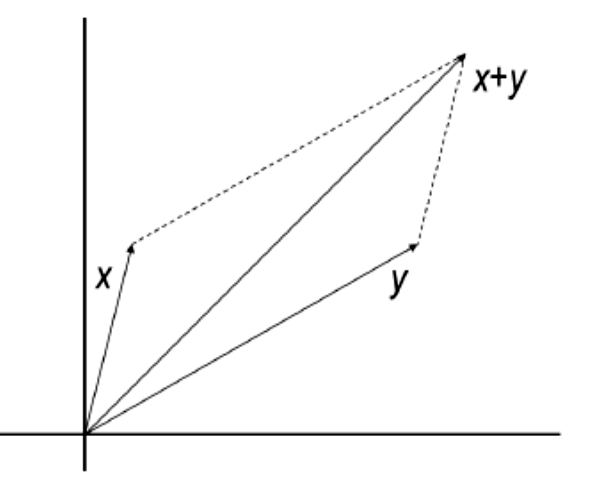
\includegraphics[scale=0.2]{media/desigualdadtriangular.png}

Las siguientes normas son las que vamos a utilizar.

\begin{ndef}[Norma p]
Sean E = $\mathbb{R}^N$, p $\geq$ 1 y x $\in$ $\mathbb{R}^N$, entonces:
\[ \Vert x \Vert _{p} := \left( \sum_{j=1}^{N} \vert x_{j} \vert ^p \right) ^{1/p} \]
Si p = 2, entonces la norma es $\textbf{euclídea}$.
\end{ndef}

\begin{ndef}[Norma del máximo]
Sea E = $\mathbb{R}^N$ y x $\in$ $\mathbb{R}^N$, entonces:
\[ \Vert x \Vert _{\infty} := max \lbrace \vert x_{j} \vert : j = 1,...,N \rbrace \]
\end{ndef}

\begin{ndef}[Norma de Frobenius]
Sea E = $\mathbb{R}^{M \times N}$ y A $\in$ $\mathbb{R}^{M \times N}$, entonces:
\[ \Vert A \Vert _F := \sqrt{\sum_{i=1}^{M} \sum_{j=1}^{N} a_{ij}^2} \]
\end{ndef}

$\textit{Aclaración:}$\\
$\textit{Si estamos en un espacio vectorial real C([a,b]), esto significa que este espacio está compuesto por todas las funciones}\\
\textit{continuas en el intervalo cerrado [a,b].}$\\
$\textit{Si el espacio es $C^k$([a,b]), significa que está formado por las funciones de clase k, es decir, funciones derivables hasta}\\
\textit{orden k y esas derivadas son continuas.}$

\begin{ndef}[Norma del máximo]
Sea E = C([a,b]) y f $\in$ C([a,b]), entonces:
\[ \Vert f \Vert _\infty := max \; \left\lbrace \vert f(x) \vert : a \leq x \leq b \right\rbrace \]
\end{ndef}

\begin{ndef}
Sean E = $C^k$([a,b]), k $\in$ $\mathbb{N}$ y f $\in$ $C^k$([a,b]) entonces:
\[ \Vert f \Vert _k := max \; \left\lbrace \Vert f^{(j)} \Vert : j = 0,...,k \right\rbrace \]
\end{ndef}

Ahora que ya tenemos definidas las normas, podemos calcular el error cometido al aproximar los vectores.

\begin{ndef}[Error absoluto]
Sea E un espacio normado, x $\in$ E y x* $\in$ una aproximación de x, entonces la siguiente operación calcula el error absoluto:
\[ \Vert x^* - x \Vert \]
\end{ndef}

\begin{ndef}[Error relativo]
Sea E un espacio normado, x $\in$ E y x* $\in$ una aproximación de x, entonces la siguiente operación calcula el error relativo:
\[  \frac {\Vert x^* - x \Vert}{ \Vert x \Vert} \]
\end{ndef}

Veamos una aplicación de estos errores.

\begin{ejer}
Calcula los errores absolutos y relativos de:
	\begin{nlist}
	\item E = $\mathbb{R}$, x = 1/4, x* = 0.23
	\item E = $\mathbb{R}^3$, x = (1/5,2,1), x* = (0.19,2.2,0.9)
	\item E = C([0,$\pi$/2]), f(t) = sen(t), f*(t) = t
	\end{nlist}
\end{ejer}

\begin{sol} $\newline$
	\begin{nlist}
	\item error absoluto: $\vert x^* - x \vert = \vert 0.23 - 1/4 \vert = 0.02 $\\
	error relativo: $\frac{\vert x^* - x \vert}{\vert x \vert} = \frac{\vert 0.23 - 1/4 \vert}{\vert 1/4 \vert} = 0.08$
	\item error absoluto: $\Vert x^* - x \Vert _\infty = \Vert (0.19,2.2,0.9) - (1/5,2,1) \Vert _\infty = \Vert (-0.01,0.2,-0.1) \Vert _\infty =$\\ $= max \lbrace 0.01,0.2,0.1\rbrace = 0.2 $\\
	error relativo: $\frac{\Vert x^* - x \Vert _\infty}{\Vert x \Vert _\infty} = \frac{\Vert (-0.01,0.2,-0.1) \Vert _\infty}{\Vert (1/5,2,1) \Vert _\infty} = \frac{0.2}{2} = 0.1 $\\
	\item error absoluto: $\Vert f^* - f \Vert _\infty = \Vert t - sen(t) \Vert _\infty = \frac{\pi}{2} - 1$\\
	error relativo: $\frac{\Vert f^* - f \Vert _\infty}{\Vert f \Vert _\infty} = \frac{\pi}{2} - 1 $
	\end{nlist}
\end{sol}

\begin{ndef}[Distancia]
Se define la $\textbf{distancia}$ entre dos vectores x,y $\in$ E como
\[ dist(x,y) := \Vert x - y \Vert \]
\end{ndef}

\begin{ndef}
Se dice que $\lbrace x_n \rbrace _{n \geq 1}$ en E $\textbf{converge}$ a $x_0$ $\in$ E sii
\[ \forall \varepsilon > 0 \Rightarrow \left[ \exists n_0 \in \mathbb{N} : n \geq n_0 \Rightarrow \Vert x_n - x_0 \Vert < \varepsilon \right] \]
es decir,
\[ \lim_{n \rightarrow \infty} x_n = x_0  \Leftrightarrow \lim_{n \rightarrow \infty} \Vert x_n - x_0 \Vert = 0 \]
\end{ndef}

\begin{ndef}
Sean X, Y subconjuntos no vacíos de sendos espacios normados y sea f: X $\rightarrow$ Y, diremos que f es $\textbf{continua}$ en $x_{0}$ $\in$ X si
\[ \forall \varepsilon > 0 \Rightarrow \left[ \exists \delta > 0 : x \in X \wedge \Vert x - x_0 \Vert < \delta \Rightarrow \Vert f(x) - f(x_0) \Vert < \varepsilon \right] \]
\end{ndef}

\begin{nprop}
Sea x $\in \mathbb{R}^N \Rightarrow \Vert x \Vert _\infty \leq \Vert x \Vert _1 \leq N\Vert x \Vert _\infty $ 
\end{nprop}

\begin{ndef}
Sean $\Vert$ · $\Vert$ y $\Vert$ · $\Vert _*$ dos normas, se dice que son $\textbf{equivalentes}$ si $\exists c_1, c_2 > 0$ tales que
\[ \forall x \in E \Rightarrow c_1\Vert x \Vert \leq \Vert x \Vert _* \leq c_2\Vert x \Vert \] 
\end{ndef}

\begin{nprop}
Sean $\Vert$ · $\Vert$ y $\Vert$ · $\Vert _*$ dos normas, entonces la convergencia de sucesiones y la continuidad son equivalentes para ambas normas. 
\end{nprop}

\begin{nth}
Todas las normas en un espacio normado finito dimensional son equivalentes.
\end{nth}

Observemos que para calcular el límite de la norma del máximo, tenemos que calcular el límite de cada coordenada.

\begin{nprop}
Sea $\mathbb{R}^N$ un espacio normado finito dimensional y consideremos la norma $\Vert$·$\Vert _\infty$ en este espacio, entonces:
\[ \lim_{n \rightarrow \infty}x_n = x_0 \Leftrightarrow \lim_{n \geq 1}(x_n)_j = (x_0)_j \qquad \forall j\in \lbrace 1,...,N \rbrace \]
\end{nprop}

\begin{proof}
\[ \lim_{n \rightarrow \infty} x_n = x_0 \quad \Leftrightarrow \quad \lim_{n \rightarrow \infty} \Vert x_n - x_0 \Vert _\infty = 0 \quad \Leftrightarrow \quad 0 < max \; \lbrace \vert (x_n - x_0)_j \vert : j = 1,...,N \rbrace = 0 \quad \rightarrow \quad \lim_{n \geq 1}(x_n)_j = (x_0)_j \]
\end{proof}

Un ejemplo de aplicación de esta proposición es el siguiente.

\begin{ejemplo}
$\lim_{n \geq 1} \left( \left( 1 + \frac{1}{n} \right) ^n , \frac{(-1)^n}{n^2} \right) = (e,0)$
\end{ejemplo}

La anterior proposición también se puede aplicar para cualquier norma de $\mathbb{R}^N$ y de $\mathbb{R}^{M \times N}$.

\begin{ejer}
Comprueba que la norma del máximo en C([0,1]) no es equivalente a la norma $\Vert$·$\Vert _1$ definida para cada f $\in$ C([0,1]) como
\[ \Vert f \Vert _1 := \int_0^1 \vert f(x) \vert dx \]
(Indicación: para cada n $\geq$ 2, considera la función $f_n$ cuya gráfica es la poligonal que une los puntos (0,0), (1/n,1), (2/n,0), (1,0)).
\end{ejer}

\begin{sol}
Tenemos que\\
\[ E = C([0,1]) \]
\[ \Vert f \Vert _\infty = max \left\lbrace \vert f(x) \vert : 0 \leq x \leq 1 \right\rbrace \]
\[ \Vert f \Vert _1 := \int_0^1 \vert f(x) \vert dx \]
Luego\\
$\Vert f_n \Vert _\infty = 1$ y $\Vert f_n \Vert _1 = 1/n$ (que coincide con el área).\\
Si fueran equivalentes, entonces
\[ \exists \alpha , \beta > 0 f \in E \Rightarrow \alpha \Vert f_n \Vert _1 \leq \Vert f_n \Vert _\infty \leq \beta \Vert f_n \Vert _1 \]
Lo cual es una contradicción, porque n $\geq$ 1 $\Rightarrow \Vert f_n \Vert _\infty \leq \beta \Vert f_n \Vert _1 \Leftrightarrow 1 \leq \frac{\beta}{n} \Leftrightarrow n \leq \beta$ $\;$ y n no está acotada.\\
Por lo que no son equivalentes.
\end{sol}

\begin{nprop}
Sean M, N $\in$ $\mathbb{N}$ y consideremos sendas normas en $\mathbb{R}^N$ y $\mathbb{R}^M$, que sin lugar a ambigüedad notaremos indeferentemente como $\Vert$·$\Vert$. Entonces la aplicación que notaremos igualmente como $\Vert$·$\Vert$ define una norma en $\mathbb{R}^{M \times N}$:
\[ \Vert A \Vert := sup \; \left\lbrace \Vert Ax \Vert : x \in \mathbb{R}^N \wedge \Vert x \Vert = 1 \right\rbrace \qquad \forall A \in \mathbb{R}^{M \times N} \]
\end{nprop}

\begin{ndef}
Se define la norma \textbf{inducida} en $\mathbb{R}^{M \times N}$ como:
\[ \Vert A \Vert := sup \; \left\lbrace \Vert Ax \Vert : x \in \mathbb{R}^N \wedge \Vert x \Vert = 1 \right\rbrace \qquad \forall A \in \mathbb{R}^{M \times N} \]
\end{ndef}

\begin{nprop}
Con la notación de la proposición anterior, si $A \in \mathbb{R}^{M \times N}$ entonces
\[ \Vert A \Vert := sup \; \left\lbrace \frac{\Vert Ax \Vert}{\Vert x \Vert } : x \in \mathbb{R}^N \wedge x \neq 0 \right\rbrace \]
En particular,
\[ \Vert Ax \Vert \leq \Vert A \Vert \Vert x \Vert \]
\end{nprop}

\begin{nprop}
Consideremos la norma $\Vert$·$\Vert _1$ en $\mathbb{R}^N$ y en $\mathbb{R}^M$, entonces la norma $\Vert$·$\Vert _1$ inducida en $\mathbb{R}^{M \times N}$ es
\[ \Vert A \Vert _1 = max \; \left\lbrace \sum_{i=1}^M \vert a_{ij} \vert : j = 1,...,N \right\rbrace \qquad \forall A \in \mathbb{R}^{M \times N} \]
\end{nprop}

Es decir, es el máximo de las sumas de los valores absolutos de cada $\textbf{columna}$.

\begin{proof} Vamos a demostrar que es $\geq$ y $\leq$, luego se dará la igualdad.\\
Probaremos primero que $ \Vert A \Vert _\infty \geq max \; \left\lbrace \sum_{j=1}^N \vert a_{ij} \vert : i = 1,...,M \right\rbrace $\\
Sea sign(a) := $\left\{ \begin{array}{lcc}
-1 & si & a < 0 \\
1 & si & a \geq 0
\end{array}
\right.$ $\qquad$ $\forall a \in \mathbb{R}$\\
Tenemos que
\[ \left\Vert \left[ sign(a_{11}),...,sign(a_{1N}) \right] ^T \right\Vert _\infty = 1 \qquad \Rightarrow \qquad \Vert A \Vert _\infty \geq \left\Vert A \left[ sign(a_{11}),...,sign(a_{1N}) \right] ^T \right\Vert _\infty \geq \sum_{j=1}^N \vert a_{1j} \vert \]
Hacemos lo mismo con $\left[ sign(a_{i1}),...,sign(a_{iN}) \right] ^T \; \forall i = 2,...,M$ y obtenemos que
\[ \Vert A \Vert _\infty \geq max \; \left\lbrace \sum_{j=1}^N \vert a_{ij} \vert : i = 1,...,M \right\rbrace \]
Ahora probaremos que $ \Vert A \Vert _\infty \leq max \; \left\lbrace \sum_{j=1}^N \vert a_{ij} \vert : i = 1,...,M \right\rbrace $\\
Sea x $\in \mathbb{R}^N$ tal que $\Vert x \Vert _\infty = 1$, entonces:
\[ \Vert Ax \Vert _\infty = \left\Vert 
\begin{bmatrix} 
a_{11} &  \cdots & a_{1N} \\
\vdots & & \vdots 
\\ a_{M1} & \cdots & a_{MN} \\ \end{bmatrix} 
\begin{bmatrix}
x_1 \\
\vdots \\
x_N \\
\end{bmatrix}
\right\Vert _\infty = \left\Vert 
\begin{bmatrix}
\sum_{j=1}^N a_{1j}x_j & ,\ldots , & \sum_{j=1}^N a_{Mj}x_j 
\end{bmatrix} ^T
\right\Vert _\infty = \] \[= max \; \left\lbrace \vert \sum_{j=1}^N a_{ij}x_j \vert : i = 1,...,M \right\rbrace \leq max \; \left\lbrace \sum_{j=1}^N \vert a_{ij} \vert \vert x_j \vert : i = 1,...,M \right\rbrace \leq \] \[ \leq max \; \left\lbrace \sum_{j=1}^N \vert a_{ij} \vert : i = 1,...,M \right\rbrace \] 
\end{proof}

\begin{nprop}
Consideremos la norma $\Vert$·$\Vert _\infty$ en $\mathbb{R}^N$ y en $\mathbb{R}^M$, entonces la norma $\Vert$·$\Vert _\infty$ inducida en $\mathbb{R}^{M \times N}$ es
\[ \Vert A \Vert _\infty = max \; \left\lbrace \sum_{j=1}^N \vert a_{ij} \vert : i = 1,...,N \right\rbrace \qquad \forall A \in \mathbb{R}^{M \times N} \]
\end{nprop}

Es decir, es el máximo de las sumas de los valores absolutos de cada $\textbf{fila}$.\\

Por lo que si ya hemos calculado alguna de estas dos últimas normas, podemos saber la otra sin tener que volver a calcular el máximo, es decir, la relación entre ambas viene en la siguiente proposición.

\begin{nprop}
$\Vert A \Vert _1 = \Vert A^T \Vert _\infty \qquad \forall A \in \mathbb{R}^{M \times N}$
\end{nprop}

Hay que tener en cuenta que $\Vert$ · $\Vert _2$ no induce en $\mathbb{R}^{M \times N}$ Frobenius.\\

Además, para las matrices $\textbf{cuadradas}$ tenemos la siguiente definición.

\begin{ndef}[Radio espectral]
Sea $A \in \mathbb{R}^{N \times N}$, denotaremos como $\textbf{radio espectral de A}$ a:
\[ \rho (A) := max \; \left\lbrace \vert \lambda \vert : \lambda \in \mathbb{C} \wedge det(A - \lambda I) = 0 \right\rbrace \]
\end{ndef}

La siguiente proposición muestra una manera más fácil de calcular la norma euclídea de un vector de $\mathbb{R}^N$, que es calculando la suma de las coordenadas al cuadrado.

\begin{nprop}
$\Vert x \Vert _2 = \sqrt{x^Tx} \qquad \forall x \in \mathbb{R}^N$
\end{nprop}

\begin{ndef}
Sea A $\in \mathbb{R}^{N \times N}$, diremos que A es $\textbf{semidefinida positiva} \Leftrightarrow x^TAx \geq 0 \qquad \forall x \in \mathbb{R}^N $
\end{ndef}

Las matrices semidefinidas positivas tienen la siguiente propiedad.

\begin{nprop}
Sea A $\in \mathbb{R}^{N \times N}$ semidefinida positiva. Si $\lambda$ es un valor propio de A $\Rightarrow \lambda \geq 0$.
\end{nprop}

\begin{proof}
Como $\lambda$ es valor propio de A $\Rightarrow \exists x \in \mathbb{R}^N : x \neq 0 \wedge Ax = \lambda x$\\
Luego\\
\[ 0 \leq x^TAx = x^T \lambda x = \lambda x^Tx = \lambda \Vert x \Vert _2^2 \]
Como x $\neq$ 0 $\Rightarrow 0 \leq \lambda$
\end{proof}

\begin{nprop}
Sea P $\in \mathbb{R}^{N \times N}$ una matriz ortogonal, entonces
\[ \left\lbrace x \in \mathbb{R}^N : \Vert x \Vert _2 = 1 \right\rbrace = \left\lbrace P^Tx : x \in \mathbb{R}^N \wedge \Vert x \Vert _2 = 1 \right\rbrace \]
\end{nprop}

\begin{proof}
Vamos a demostrar la doble inclusión, lo que dará la igualdad.\\
$\textbf{¿ $\supseteq$ ?}$\\
Sea $x \in \mathbb{R}^N : \Vert x \Vert _2 = 1 \; \Rightarrow \;$ ¿ $\Vert P^Tx \Vert _2 = 1 $ ?
\[ \Vert P^Tx \Vert _2 = \sqrt{x^TPP^Tx} = \sqrt{x^Tx} = \Vert x \Vert _2 = 1 \]
$\textbf{¿ $\subseteq$ ?}$\\
\[ 1 = \Vert x \Vert _2 = \sqrt{x^Tx} = \sqrt{x^TIx} = \sqrt{x^TPP^Tx} = \Vert P^Tx \Vert _2 \]
\end{proof}

\begin{nprop}
Si $\lambda _1,..., \lambda _N \geq 0 \Rightarrow sup \; \left\lbrace \sqrt{\sum_{i=1}^N \lambda _iy_i^2} : y \in \mathbb{R}^N \wedge \Vert y \Vert _2 = 1 \right\rbrace = \sqrt{max \; \lambda _i : i = 1,...,N} $
\end{nprop}

\begin{proof}
\end{proof}

Una manera más sencilla de calcular la norma de una matriz es la siguiente.

\begin{nprop}
Sea A $\in \mathbb{R}^{M \times N} \Rightarrow \Vert A \Vert _2 = \sqrt{\rho (A^TA)} $
\end{nprop}

\begin{ndef}[Norma matricial]
Una norma en $\mathbb{R}^{N \times N}$ se dice $\textbf{matricial}$ cuando
\[ \Vert AB \Vert \leq \Vert A \Vert \Vert B \Vert \qquad \forall A,B \in \mathbb{R}^{N \times N} \]
\end{ndef}

Hay que tener en cuenta de que no toda norma en $\mathbb{R}^{N \times N}$ es matricial, por ejemplo:\\
Vamos a utilizar la siguiente norma\\
$\Vert A \Vert := max \; \lbrace \vert a{ij} \vert : i, j = 1,...,N \rbrace \qquad \forall A \in \mathbb{R}^{N \times N}$ \\
Sean A = B = $\begin{bmatrix}
1 & 1 \\
1 & 1 \\
\end{bmatrix}$\\
Luego tenemos que
$2 = \Vert AB \Vert > \Vert A \Vert \Vert B \Vert = 1$\\
Por lo que esta norma no es matricial.\\

\begin{nprop}
Toda norma en $\mathbb{R}^{N \times N}$ inducida por una norma en $\mathbb{R}^N$ es matricial.
\end{nprop}

\begin{proof}
Sea $\Vert$ · $\Vert$ una norma en $\mathbb{R}^{N \times N}$ inducida por una norma en $\mathbb{R}^N$, entonces
\[ \Vert A \Vert := sup \; \left\lbrace \Vert Ax \Vert : x \in \mathbb{R}^N \wedge \Vert x \Vert = 1 \right\rbrace \]
Sabemos que la norma es inducida, luego se cumple que
\[ \Vert Ax \Vert \leq \Vert A \Vert \Vert x \Vert \qquad \forall x \in \mathbb{R}^N \]
Tenemos que probar que $\Vert AB \Vert \leq \Vert A \Vert \Vert B \Vert$\\
\[ \Vert AB \Vert = sup \; \left\lbrace \Vert ABx \Vert : x \in \mathbb{R}^N \wedge \Vert x \Vert = 1 \right\rbrace \leq sup \; \left\lbrace \Vert A \Vert \Vert Bx \Vert : x \in \mathbb{R}^N \wedge \Vert x \Vert = 1 \right\rbrace \leq \] \[ \leq sup \; \left\lbrace \Vert A \Vert \Vert B \Vert \Vert x \Vert : x \in \mathbb{R}^N \wedge \Vert x \Vert = 1 \right\rbrace = \Vert A \Vert \Vert B \Vert \]
\end{proof}

\begin{nth}
$\lim_{n \rightarrow \infty} A^n = 0 \; \Leftrightarrow \; \rho (A) < 1 \qquad \forall A \in \mathbb{R}^{N \times N} $
\end{nth}

Este teorema nos deja dos importantes consecuencias.

\begin{ncor}
Sea A $\in \mathbb{R}^{N \times N}$ una matriz triangular, entonces
\[ \lim_{n \rightarrow \infty} A^n = 0 \quad \Leftrightarrow \quad max \; \lbrace \vert a_{ii} \vert < 1 : i = 1,...,N \rbrace \]
\end{ncor}

\begin{proof}
\end{proof}

\begin{ncor}
Sean N $\geq$ 1, A $\in \mathbb{R}^{N \times N}$ y $\Vert$ · $\Vert$ una norma matricial en $\mathbb{R}^{N \times N}$ tal que $\Vert$A$\Vert$ < 1, entonces $\rho$(A) < 1
\end{ncor}

Hay que tener en cuenta que no se cumple la implicación contraria, por ejemplo:\\
Sea A = $\begin{bmatrix}
0.5 & 500 \\
0 & 0.5 \\
\end{bmatrix}$ $\Rightarrow \rho (A) = 0.5 < 1$ pero $\Vert A \Vert _\infty = 500.5 \geq 1$


\subsection{Problemas bien planteados. Estabilidad}
Nos planteamos el siguiente problema:\\
Sean X e Y subconjuntos no vacíos de sendos espacios normados reales, f: X $\rightarrow$ Y una aplicación, $y_0 \in$ Y. Entonces tenemos que encontrar $x_0 \in X : f(x_0) = y_0$\\
Denotaremos a $x_0$ como la solución que resuelve el problema determinado por f y a $y_0$ los datos, es decir, son números. Si tenemos un conjunto finito de números, usaremos el vector de $\mathbb{R}^N$ o matriz, y si tenemos infinitos datos, usaremos una función.

\begin{ejemplo}
Sean $A \in \mathbb{R}^{M \times N}$ y $y \in \mathbb{R}^M$. Determinar una solución del sistema de ecuaciones lineales cuya matriz de coeficientes sea A y su vector de términos independientes sea y\\
$X = \mathbb{R}^N$, $Y = \mathbb{R}^M$, f(x) = Ax = y
\end{ejemplo}

\begin{ndef}
Un problema está $\textbf{bien planteado}$ cuando es $\textbf{unisolvente}$ y $\textbf{estable}$:
	\begin{nlist}
	\item $\exists ! x_0 \in X : f(x_0) = y_0$.
	\item $x_0$ depende continuamente de los datos $y_0$.
	\end{nlist}
\end{ndef}

En el siguiente ejemplo veremos un problema mal planteado.

\begin{ejemplo}
Sean X := $\mathbb{R}$, Y := $\mathbb{R}_+ \;$ y $\; f(x) := \vert x \vert , \; \forall x \in X$\\
Observamos que este problema no es unisolvente, ya que si $y_0$ = 1 (lo mismo vale $\forall y_0 > 0$) tenemos que f(-1) = 1 = f(1)
\end{ejemplo}

\begin{ndef}[Resolvente]
Denotaremos a la función g como la $\textbf{resolvente}$ de f si g es la inversa de f, para todo y $\in$ Y unisolvente.
\end{ndef}

\begin{ejemplo}
Sean X := $\mathbb{R}$, Y := $\mathbb{R}_+ \;$ y $\; f(x) := e^x , \; \forall x \in X$\\
Entonces este problema es unisolvente, luego tiene resolvente: g(y) = log y, para todo y $\in$ Y.
\end{ejemplo}

Podemos ver la estabilidad de un problema intuitivamente, es decir, a pequeñas perturbaciones de los datos $y_0$ corresponden pequeñas perturbaciones de la solución $x_0$.

\begin{ejemplo}
Consideremos el problema X := [-1,1] =: Y, $\;$
$
f(x) := \left\{ \begin{array}{lcc}
x & si & -1 < x < 1 \\
\\ -x & si & x = \pm 1
\end{array}
\right.
$.\\
Entonces este problema es unisolvente, ya que la función f :  [-1,1] $\rightarrow$ [-1,1] es biyectiva y g = f.\\
Pero para que esté bien planteado, tiene que ser, además, estable. Veamos que no es estable, ya que a pequeñas perturbaciones del dato $y_0$ = -1 (lo mismo con $y_0$ = 1) no corresponden pequeñas perturbaciones de $x_0$ = 1.\\
Sea $y_n := -1 + \frac{1}{n} \rightarrow y_0 = -1$, entonces $g(y_n) = -1 + \frac{1}{n} \rightarrow -1$, ya que $y_n = g(y_n)$.\\
Luego $\vert -1 - x_0 \vert = 2$, es decir, las perturbaciones de $x_0$ son muy grandes.
\end{ejemplo}

Ahora nos planteamos la siguiente cuestión: ¿La estabilidad del problema y la continuidad de la resolvente g tienen algo que ver? Veamos en el siguiente ejemplo que no siempre es así.

\begin{ejemplo}
Consideremos el problema $f : \mathbb{R}_+ \rightarrow \mathbb{R}_+, f(x) := \left( \frac{x}{10} \right) ^10 \; \forall x \geq 0$.\\
Tenemos que este problema es unisolvente y su resolvente es $g : \mathbb{R}_+ \rightarrow \mathbb{R}_+, g(y) = 10y^{\frac{1}{10}} \; \forall y \geq 0$.\\
Tenemos que g es continua, luego pequeños cambios de los datos $y \in \mathbb{R}_+$ nos llevan a cambios cercanos de las correspondientes soluciones $x \in \mathbb{R}_+$ pero no controlados, se aproximan a una velocidad diferente. Vamos a comprobarlo.\\
Tenemos que $y_0 = 0 = x_0$. Sea y un dato próximo a $y_0$, por ejemplo y = $10^{-10}$. Entonces la solución correspondiente es $x = g(y) = 10y^{\frac{1}{10}} = 10 \cdot \left( 10^{-10} \right) ^{\frac{1}{10}} = \frac{10}{10} = 1$. Por lo que tenemos lo siguiente:\\
$\vert y - y_0 \vert = 10^{-10}$, $\vert x - x_0 \vert = 1$.\\
Es decir, el número $10^{-10}$ indica la velocidad con la que se mueven los datos y, en comparacion con el número 1, que indica que los datos x se mueven mucho más rápido, lo que nos lleva a que, aunque g sea continua, la velocidad de aproximación es diferente, luego no hay estabilidad.
\end{ejemplo}

Luego podríamos decir que la estabilidad es una condición que fuerce un control de los valores de las soluciones en función de los datos, de forma que pequeñas perturbaciones de $y_0$ generen perturbaciones pequeñas y controladas de $x_0$.

\begin{ndef}
Sean X e Y subconjuntos no vacíos de sendos espacios normados, $g : Y \rightarrow X$ una aplicación e $y_0 \in Y$. Diremos que g es $\textbf{estable}$ en $y_0$ cuando
 \[ \exists \delta , M > 0 : sup \; \left\lbrace \frac{ \Vert g(y) - g(y_0) \Vert }{ \Vert y - y_0 \Vert } : y \in Y \wedge 0 < \Vert y - y_0 \Vert < \delta \right\rbrace < M \]
y que g es $\textbf{estable}$ si lo es en todos y cada uno de los elementos de Y.
\end{ndef}

\begin{ndef}
Un problema es $\textbf{estable en $y_0 \in$ Y}$ si su resolvente $g : Y \rightarrow X$ lo es en dicho punto, y es $\textbf{estable}$ si lo es en cualquier dato de Y.
\end{ndef}

Habrá mejor comportamiento cuanto más pequeño sea M.

\begin{nprop}
g es estable en $y_0 \Rightarrow$ g es continua en $y_0$ 
\end{nprop}

Veamos que la implicación $\nLeftarrow$ se cumple al tomar la resolvente del ejemplo anterior en 0, o si se quiere, la función raíz cuadrada en 0.\\

\begin{nprop}
Toda función real de variable real de clase $C^1$ es estable.
\end{nprop}

Para demostrar esta proposición hay que usar el Teorema del Valor Medio. Además, el recíproco no es cierto.\\
Sea f una función de variable real de clase $C^1$, vamos a medir su estabilidad en $x_0 \in \mathbb{R}$.\\
Si $x_0f(x_0) \neq 0$, entonces el cociente entre el error relativo cometido cerca de $f(x_0)$ y el error relativo de $x_0$ es:
\[ \left\vert \frac{\frac{f(x) - f(x_0)}{f(x_0)}}{\frac{x - x_0}{x_0}} \right\vert = \left\vert \frac{f(x) - f(x_0)}{x - x_0} \right\vert \left\vert \frac{x_0}{f(x_0)} \right\vert \]
Si $x_0f(x_0) = 0$, entonces los errores absolutos cerca de $f(x_0)$ e $x_0$ es:
\[ \left\vert \frac{f(x) - f(x_0)}{x - x_0} \right\vert \]

De forma precisa:

\begin{ndef}
Dada una función $f \in C^1(\mathbb{R})$ y un punto $x_0 \in \mathbb{R}$, el $\textbf{condicionamiento relativo}$ de f en $x_0$ viene dado por
\[ c(f, x_0) := \left\vert \frac{f'(x_0)x_0}{f(x_0)} \right\vert \]
siempre que $x_0f(x_0) \neq 0$.\\
En caso contrario, el $\textbf{condicionamiento absoluto}$ de f en $x_0$ es
\[ C(f, x_0) := \vert f'(x_0) \vert \]
\end{ndef}

Ídem en funciones reales de variable real definidas en intervalos de $\mathbb{R}$ y de clase $C^1$.\\
Para calcular el condicionamiento en funciones de varias variables, usamos lo siguiente:
\[ c(f,x_0) := \frac{\left\Vert \frac{\partial f}{\partial x} (x_0) \right\Vert \Vert x_0 \Vert}{\Vert f(x_0) \Vert} \]
\[ C(f,x_0) := \left\Vert \frac{\partial f}{\partial x} (x_0) \right\Vert \]

\begin{ndef}
Si en un problema la resolvente s de clase $C^1$ e $y_0 \in Y$, el $\textbf{condicionamiento relativo}$ o $\textbf{absoluto}$ del problema son los de su resolvente en dicho punto.
\end{ndef}

\begin{nota}
Aunque se trata de un concepto bastante ambiguo, suele decirse que una aplicación (o un problema) está $\textbf{bien condicionado}$ en un punto si su condicionamiento es pequeño y en caso contrario, $\textbf{mal condicionado}$.
\end{nota}

\begin{ejemplo}
Sea $f : (0,1) \rightarrow (0, \pi / 2), \; f(x) := arcsen(x)$.\\
Veamos si está bien planteado.\\
La resolvente es $g : (0, \pi / 2) \rightarrow (0,1), \; g(y) := sen(y)$. Luego está bien planteado.\\
Veamos si está bien condicionado.\\ Para ello calculamos el condicionamiento relativo en $y_0 \in (0, \pi / 2)$.\\
\[ c(g,y_0) = \frac{\vert g'(y_0)y_0 \vert }{\vert g(y_0) \vert} = y_0 \frac{cos(y_0)}{sen(y_0)} \]
Como $c(g,y_0) \in (0,1) \Rightarrow$ está bien condicionado.
\end{ejemplo}

\begin{ejemplo}
Sea $A \in \mathbb{R}^{N \times N}$ regular e $y \in \mathbb{R}$, encuentra $x \in \mathbb{R}^N$ : f(x) = y.\\
Sea f(x) = Ax, como A es regular, es unisolvente el problema, luego tiene resolvente $g : \mathbb{R}^N \rightarrow \mathbb{R}^N$, $g(y) := A^{-1}y, \; \; \forall y \in \mathbb{R}^N$\\
Además, el problema es estable en todo $y_0 \in \mathbb{R}^N$, ya que:
\[ \Vert g(y) - g(y_0) \Vert _\infty \leq \Vert A^{-1} \Vert _\infty \Vert y - y_0 \Vert _\infty \]
Ahora calcularemos el condicionamiento relativo.
\[ c(g, y_0) = \frac{\Vert \frac{\partial g}{\partial y} (y_0) \Vert \Vert y_0 \Vert }{\Vert g(y_0)} = \frac{\Vert A^{-1} \Vert \Vert y_0 \Vert }{\Vert A^{-1} y_0 \Vert } = \frac{\Vert A^{-1} \Vert \Vert y_0 \Vert }{\Vert x_0 \Vert } \] 
Luego $Ax_0 = y_0$
\end{ejemplo}

Si $\Vert A^{-1} \Vert$ es grande, $x_0$ e $y_0$ son del mismo orden, entonces el condicionamiento será grande. Observémoslo en el siguiente ejemplo.

\begin{ejemplo}
Sea $A = \begin{bmatrix}
1 & 1 \\
1 & 0.999 \\
\end{bmatrix}$,
un dato $y_0 = \begin{bmatrix}
2 \\
1.999 \\
\end{bmatrix}$
y su solución $x_0 = \begin{bmatrix}
1 \\
1 \\
\end{bmatrix}$\\

Veamos que hay un mal condicionamiento, ya que el condicionamiento es demasiado grande en comparación con el resto. Para ello, calculamos antes la inversa de la matriz A y la norma del máximo de esta, de la solución $x_0$ y del dato $y_0$.

\[ A^{-1} = \begin{bmatrix}
-999 & 1000 \\
1000 & -1000 \\
\end{bmatrix} \]
\[ \Vert A^{-1} \Vert _\infty = 2000, \; \; \Vert x_0 \Vert _\infty = 1, \; \; \Vert y_0 \Vert _\infty = 2 \]
Luego el condicionamiento se calculará con la expresión obtenida anteriormente usando la norma infinito.
\[ c(g, y_0) = \frac{\Vert A^{-1} \Vert _\infty \Vert y_0 \Vert _\infty }{\Vert x_0 \Vert _\infty } = 4000 \]
Como hemos dicho, es un condicionamiento demasiado grande y nos preguntamos ¿cuál es el problema? Pues que al calcular las soluciones de otros datos próximos al inicial, las soluciones obtenidas no son próximas a la solución inicial. Comprobémoslo.\\
Sea y un dato próximo a $y_0$, por ejemplo $y = \begin{bmatrix}
2 \\
1.998 \\
\end{bmatrix}$.
Es próximo, ya que $\Vert y - y_0 \Vert _\infty = 0.001$.\\
Su solución es $x = A^{-1}y = \begin{bmatrix}
0 \\
2 \\
\end{bmatrix}$. No es próxima a la solución inicial, ya que $\Vert x - x_0 \Vert _\infty = 1$\\
La interpretación geométrica de este resultado es: las columnas de A forman base de $\mathbb{R}^{2 \times 2}$, calculamos las coordenadas de y en $y_0$ en dicha base. Un pequeño cambio entre y e $y_0$ genera un cambio grande de coordenadas por ser los vectores de la base casi paralelos.
\end{ejemplo}

Ahora nos planteamos la siguiente pregunta: ¿está globalmente acotado el condicionamiento relativo de un sistema de cuaciones lineales? La respuesta es afirmativa y nos da una idea de cómo de estable es.\\

La siguiente definición será útil para calcular el condicionamiento de una matriz cuando la norma es inducida.

\begin{ndef}
Si $\Vert \cdot \Vert$ denota la norma matricial en $\mathbb{R}^{N \times N}$ inducida por una norma en $\mathbb{R}^N$, que notaremos igualmente como $\Vert \cdot \Vert$, entonces definimos el $\textbf{condicionamiento}$ c(A) de una matriz regular A $\in \mathbb{R}^{N \times N}$ como
\[ c(A) := \Vert A^{-1} \Vert \Vert A \Vert \]
\end{ndef}

Además,
\[ sup \; \left\lbrace c(g, y_0) : y_0 \neq 0 \right\rbrace = sup \; \left\lbrace \frac{\Vert A^{-1} \Vert \Vert y_0 \Vert}{\Vert A^{-1}y_0 \Vert} : y_0 \neq 0 \right\rbrace = sup \; \left\lbrace \frac{\Vert A^{-1} \Vert \Vert Ax_0 \Vert}{\Vert x_0 \Vert} : x_0 \neq 0 \right\rbrace = \Vert A^{-1} \Vert \Vert A \Vert \]

Lo que nos lleva a que si tenemos un mal condicionamiento del sistema, el condicionamiento de la matriz de coeficientes es grande, y viceversa.\\
También tenemos que $c(A) \geq 1$.\\
Si retomamos el ejemplo anterior, usando la norma del máximo en $\mathbb{R}^2$ y la correspondiente norma matricial inducida, obtenemos que c(A) = 4000.

\subsection{Algoritmos. Algoritmo PageRank de Google}

\begin{ndef}[Algoritmo]
Procedimiento que describe de forma precisa, y siempre mediante un número finito de operaciones aritméticas y lógicas elementales, la resolución de un problema.
\end{ndef}

El algoritmo recoge las instrucciones que permiten al ejecutor del mismo resolver completamente el problema. El ejecutor suele ser un ordenador y, de hecho, en la mayoría de los casos, no puede ser una persona.

\begin{ndef}[Análisis Numérico]
Se ocupa de diseñar algoritmos que permitan la resolución efectiva de problemas bien planteados y que involucran números reales.
\end{ndef}

\begin{ndef}[Complejidad de un algoritmo]
Medida del tiempo de ejecución y que suele expresarse en términos de un parámetro asociado al problema.
\end{ndef}

Al desarrollar y analizar un algoritmo obtenemos precisión, estabilidad y efectos de la representación finita de los números reales.

El Algoritmo PageRank de Google mide la relevancia de las páginas web (dominios...) con enlaces en común. Por lo que aquí nuestro problema es calcular la relevancia de una página (P), teniendo en cuenta el número de enlaces de otras páginas a (P) y la importancia de las páginas que establecen enlace con (P).

Nuestro modelo es:\\
Denotaremos al conjunto (finito) de páginas web como 1, 2, ..., $x_N$.\\
Denotaremos a las páginas como 1, 2, ..., i.\\
La relevancia de la página i se representa por $x_i \geq 0$.\\
La página i será más importante que la página j si $x_i > x_j$.

\begin{ejemplo}
%Insertar imagen
La relevancia de cada página será la suma de los cocientes entre la relevancia de la página que entra y los enlaces que salen de esta.
\[ x_1 = \frac{x_3}{3}, \; \; x_2 = \frac{x_1}{3} + \frac{x_3}{3} + \frac{x_4}{2}, \; \; x_3 = \frac{x_1}{3} + \frac{x_1}{3} + \frac{x_4}{2}, \; \; x_4 = \frac{x_1}{3} + x_2 + \frac{x_3}{3} \]

Por lo que siempre obtendremos un sistema compatible indeterminado con un parámetro.\\

Si tomamos $x_4$ como parámetro y le asignamos el valor 10, tenemos lo siguiente:
\[ x_1 = 1.875, \; \; x_2 = 7.5, \; \; x_3 = 5.625, \; \; x_4 = 10 \]
\end{ejemplo}

\section{Errores de redondeo. Iteradores}
Las principales fuentes de error suelen ser equivocarse al elegir el modelo de un problema, la medida de los datos experimentales, error al truncar o al redondear y consecuentemente, al operar, se produce una propagación del error.

\subsection{Sistema posicional y números máquina}
Los ordenadores trabajan con un subconjunto finito de números reales, los $\textbf{números máquina}$, subconjunto que depende de las especificaciones del ordenador.\\

$\textbf{SISTEMAS POSICIONALES DE NUMERACIÓN}$\\
Sea $b \in \mathbb{N}$ la base binaria o decimal, según el estándar ISO/IEC/IEEE60559:2011 del IEEE (Institute of Electrical and Electronic Engineers, www.ieee.org). Sea $s \in$ {0,1} el signo, N,M $\in \mathbb{N} \cup$ {0} y sea $x_k$ la cifra en la posición k tal que $0 \leq x_k < b, \; \; \forall k = -M, ..., N$.\\
La $\textbf{representación posicional}$ de un número real es:
\[ x = (-1)^s \sum_{n=-M}^N x_nb^n \]
\[ x_b := (-1)^s \cdot (x_N...x_1x_0.x_{-1}x_{-2}...x_{-M})_b \]
Además, denominaremos al punto entre $x_0$ y $x_{-1}$ como $\textbf{punto binario}$ o $\textbf{punto decimal}$.

\begin{ejemplo}
Sea $x_{10} = x = 101.11$, su representación posicional es x = 1·$10^2$ + 1·$10^0$ + 1·$10^{-1}$ + 1·$10^{-2}$.\\
Sea $y_2 = (101.11)_2$, su representación posicional es y = 1·$2^2$ + 1·$2^0$ + 1·$2^{-1}$ + 1·$2^{-2}$.
\end{ejemplo}

Variando $M, N \in \mathbb{N} \cup \lbrace 0 \rbrace $ tenemos un subconjunto denso de $\mathbb{R}$. Además, la serie geométrica de razón menor que 1 converge. Se puede extender a infinito:
\[ x = (-1)^s \sum_{- \infty}^N x_nb^n \]
\[ x_b := (-1)^s \cdot (x_N...x_1x_0.x_{-1}x_{-2}...)_b \]

El siguiente ejemplo aprenderemos representar en forma posicional infinita a partir de otra infinita.

\begin{ejemplo}
\[ (0.\stackrel{\large \frown}{001}) _2 = \sum_{n=1}^{\infty} \left( 2^{-3} \right) ^n = \frac{1}{7} = \stackrel{\Large \frown}{0.142857} \]
Para calcular la convergencia de esta serie, como la razón es menor que 1, hemos usado lo siguiente:
\[ \alpha \neq 1, \; n > k \geq 0 \; \; \Rightarrow \sum_{j=k}^n \alpha ^j = \frac{\alpha ^k - \alpha ^{n+1}}{1 - \alpha} \]
En particular, si \[ \vert \alpha \vert < 1 \; \; \Rightarrow  \sum_{j=k}^\infty \alpha ^k = \frac{\alpha ^k}{1 - \alpha} \]
\end{ejemplo}


\subsection{Redondeo en sistemas de punto flotante y su aritmética}


\subsection{Iteradores}


\part{Tema2}


